\section{Towards Proactive Idea in Dynamic Load Balancing and Co-scheduling Tasks}
\label{sec:Idea-Proactive-LB}
\index{PerfModel!A Proactive Idea for Load Balancing}

The previous section highlights that task migration overhead in distributed memory systems is not the only primary influence factor. Instead, balancing operation overhead can also affect our performance. The balancing operations consist of monitoring queue information or status, calculating imbalance, exchanging status information, and making decisions on task migration. The overhead of each operation might be small and trivial. However, when they are performed numerously and continuously, the decisions of task migration can be significantly impacted. Eventually, the performance of load balancing is affected overall.\\

This subsection emphasizes three representative pillars that lead to wrong decision-making for reactive load balancing in particular and dynamic load balancing in general. Figure \ref{fig:three_pillars_reactlb} shows these pillars from left to right, including:
\begin{itemize}
	\item The first pillar implies the factors of imbalance reason (in our context, slowdown is mentioned and denoted by $S_{P}$) and imbalance level ($R_{imb}$).
	\item The second pillar is related to the overhead of load monitoring ($m$) and information exchanging ($b$).
	\item The third pillar is the overhead of task offloading, indicating the delay time ($d$) when tasks are migrated.
\end{itemize}

\begin{figure}[t]
  \centering
  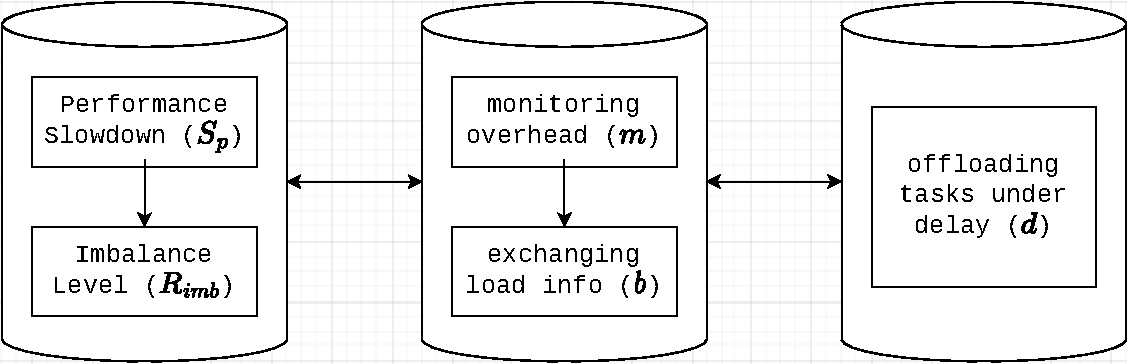
\includegraphics[scale=0.55]{./pictures/perf_analysis_model/perf_three_pillars_of_react_lb.pdf}
	\caption{Three pillars of factors might challenge reactive load balancing.}
	\label{fig:three_pillars_reactlb}
\end{figure}

Concretely, the first pillar implies imbalance context related to performance slowdown, leading to high or low imbalance levels. The second pillar is overhead in the middle, revolving around balancing operations. At runtime, all dynamic load balancing methods perform seemingly random operations before a task can be migrated. The last pillar is about overhead and decision-making for task offloading as well as task migration. If the second pillar takes a small overhead, then decisions in the third pillar can be made faster. When tasks are decided to migrate, the main overhead is delay time $d$, which $d$ is large or small, depending on the data size of tasks, latency, and network bandwidth. We describe the interaction between these pillars as follows.
\begin{itemize}
	\item If $R_{imb}$ is high, the imbalance condition might be detected in high frequency. Then, task offloading decisions are made many times.
	\item To know how many tasks and where to offload tasks, there are different ways to make decisions associated with the first pillar.
	\begin{itemize}
		\item For safety, exactly one task should be moved at one point in time. However, this might lead to many monitoring, checking, and exchanging load information operations. Simultaneously, the big enough values of $d$ can make these points challenging because it can take time to finish the exchanging operations before a task is decided for migration.
		\item To reduce the number of migration procedures, several tasks can be moved at once. However, deciding how many tasks are appropriate without prior knowledge is difficult.
	\end{itemize}
\end{itemize}

We can see that ``reactive'' load balancing implies taking actions reactively based on the most current status. This also means that we cannot plan to decide how many tasks should be migrated at a time adaptively. Besides, there is no information about which process could be a potential victim. When balancing operation and task migration produce a certain overhead, the decisions of reactive load balancing can be late and incorrect.\\

In general, we highlight that the challenge of dynamic load balancing is to obtain prior knowledge about load information. Assuming that we can predict load information or generate knowledge about load information at runtime, we can drive load balancing better. This thesis motivates an idea: How can we perform load balancing more proactively at runtime? ``Proactive'' implies that we can calculate how bad the imbalance is at a current state and how many tasks should be migrated at once. Consequently, we propose a proactive load balancing approach that enables to characterize task execution, learn load information, and predict imbalance. This is considered a better prognostication compared to the reactive load balancing approach. From idea to practice, our proactive approach is developed by the following technical questions:
\begin{itemize}
	\item Can we use a dedicated thread to obtain load values at runtime?
	\item Can we leverage the profiled information of several first iterations (or previous iterations) to generate the load knowledge?
	\item Can we change from reactive to more proactive task offloading between iterations?
\end{itemize}

For most of the use cases in HPC, iterative applications or simulation frameworks can benefit from our approach. Their behaviors are divided into multiple execution phases (so-called iterations). With a large simulation use case, a program can be run with many iterations, and an adaptive approach for load balancing is essential. Therefore, our proactive idea can be relevant to make load balancing more adaptive. The following chapter will show in detail how we design the idea.

% Taking a look at the condition for task offloading, it relies on setting an imbalance threshold and the availability of tasks at a time.